% Created 2021-08-19 Thu 09:06
% Intended LaTeX compiler: pdflatex
\documentclass[11pt]{article}
\usepackage[utf8]{inputenc}
\usepackage{lmodern}
\usepackage[T1]{fontenc}
\usepackage{fixltx2e}
\usepackage{graphicx}
\usepackage{longtable}
\usepackage{float}
\usepackage{wrapfig}
\usepackage{rotating}
\usepackage[normalem]{ulem}
\usepackage{amsmath}
\usepackage{textcomp}
\usepackage{marvosym}
\usepackage{wasysym}
\usepackage{amssymb}
\usepackage{amsmath}
\usepackage[version=3]{mhchem}
\usepackage[numbers,super,sort&compress]{natbib}
\usepackage{natmove}
\usepackage{url}
\usepackage{minted}
\usepackage{underscore}
\usepackage[linktocpage,pdfstartview=FitH,colorlinks,
linkcolor=blue,anchorcolor=blue,
citecolor=blue,filecolor=blue,menucolor=blue,urlcolor=blue]{hyperref}
\usepackage{attachfile}
\usepackage{geometry}
\geometry{margin=1.0in,top=.75in,bottom=.75in}
\usepackage{graphicx}
\usepackage{color}
\usepackage[numbers,super,sort&compress]{natbib}
\usepackage{caption}
\usepackage{subcaption}
\captionsetup{font=footnotesize}
\usepackage[version=3]{mhchem}
\usepackage{siunitx}
\usepackage{fancyhdr}
\usepackage{paralist}
\usepackage{amsmath}
\usepackage{enumitem}
\usepackage{mdwlist}
\usepackage{hyperref}
\pagestyle{fancy}
\usepackage{wrapfig}
\usepackage{nopageno}
\fancyhf{}
\fancyhead[LE,RO]{\scriptsize Jerry Crum}
\fancyhead[RE,LO]{\scriptsize ZSE Outline}
%\fancyfoot[CE,CO]{\leftmark}
\fancyfoot[LE,RO]{\thepage}
%\usepackage{subfig}
\usepackage{comment}
\usepackage{titlesec}
\titlespacing*{\section}
{0pt}{0.6\baselineskip}{0.2\baselineskip}
\titlespacing*{\subsection}
{0pt}{0.6\baselineskip}{0.2\baselineskip}
\titlespacing*{\subsubsection}
{0pt}{0.4\baselineskip}{0.1\baselineskip}
\usepackage{parskip}
\usepackage[section]{placeins}
\usepackage{siunitx}
\DeclareGraphicsExtensions{.pdf,.png,.jpg}
\newcommand{\red}[1]{\textcolor{red}{#1}}
\newcommand{\blue}[1]{\textcolor{blue}{#1}}
\newcommand{\green}[1]{\textcolor{green}{#1}}
\newcommand{\orange}[1]{\textcolor{orange}{#1}}
\usepackage[capitalise]{cleveref}
\author{Jerry T. Crum\(^{\text{a}}\), Justin R. Crum\(^{\text{b}}\), William F. Schneider\(^{\text{a,c}}\)}
\date{}
\title{ZSE Manuscript Outline}
\begin{document}

\begin{OPTIONS}
\def\udesoftecoverride\#1\mainmatter\{\%
  \AfterEndPreamble{#1\mainmatter}
\end{OPTIONS}

\maketitle

\begin{asparaenum}[\expandafter\textsuperscript a ]
\item Department of Chemical and Biolmolecular Engineering, University of Notre Dame, 250 Nieuwland Science Hall, Notre Dame, IN 46556, USA \\
\item Department of Applied Mathematics, University of Arizona, 617 N Santa Rita Ave, Tucson, AZ 85721, USA\\
\item Department of Chemistry and Biochmeistry, University of Notre Dame, 251 Nieuwland Science Hall, Notre Dame, IN 46556, USA
\end{asparaenum}

\newpage
\section*{Abstract}
\label{sec:org05df739}
The topology of zeolite frameworks and of associated tetrahedral sites (T-sites) are commonly characterized by their associated rings, typically defined as some set of closed paths or cycles through a framework that cannot be decomposed into shorter cycles. These ring descriptors have been used to identify feasible zeolite topologies, to describe the similarity and differences between zeolites, to identify sites or voids of catalytic relevance, and as machine learning fingerprints. Numerous definitions and algorithms for finding zeolite rings have been proposed and applied throughout the literature. Here we report an analysis of rings and T-sites in a large number of zeolite frameworks using Zeolite Simulation Environment, a Python package that implements an efficient algorithm presented by Goetzke and Klein for finding rings in arbitrary frameworks. We compare the result of a number of common and new ring definitions applied to a large number of common zeolite frameworks. We discover previously unrecognized rings in a number of frameworks. We show that the vertex symbol, a common approach used to characterize T-sites, misses important parts of the stereochemistry around a T-site, and propose an alternative definition. This tool provides an effective platform for characterizing zeolite and T-site structures useful for building models and doing machine learning. 


\section*{Discussion With Bill:}
\label{sec:org9bd16bb}
\begin{enumerate}
\item Go through table again to make sure we agree
\begin{enumerate}
\item Will move vertex symbol outside of table
\end{enumerate}
\item Naming the ring conventions:
\begin{enumerate}
\item Goetzke: ring, primitive ring, fundamental ring \cite{marians-network-1990,guttman-ring-1990,goetzke-properties-1991}
\item Sastre: Shortest path ring, something else?
\item Crum: Unstacked rings, something else?
\end{enumerate}
\item Look at updated highlights
\item Look at intro again
\end{enumerate}

\section*{Highlights}
\label{sec:org61c4a30}
What is the main point of the paper? What problem is it addressing? What are the main insights?

\begin{enumerate}
\item Zeolite framework and nodes commonly classified in terms of rings
\item Various conventions for associating some subsets of rings with either a framework, the T-sites of a framework, or the oxygens of a framework.
\item PROBLEM TO ADDRESS: The convention used will provide different ring counts
\item SOLUTION: We provide a Python package that has the ability to identify and classify these rings based on previously published and new conventions
\item This software tool uses a node-based search procedure that takes advantage of algorithms developed for general nets
\item We compute and compare conventions across all known frameworks
\item Some features treated by convention as rings are not rings in a topological sense but are rather defined by the void space they create.
\item We enumerate all rings, defined as paths with no short-cut, up to 18 T-sites across all known Fws
\begin{enumerate}
\item Would be very cool to classify Fws according to these rings\ldots{}.
\begin{enumerate}
\item Not sure what approach to use for that, but it is a good idea
\end{enumerate}
\item Compare to other classifications, eg cage-window vs channel
\end{enumerate}
\end{enumerate}

\section*{Introduction}
\label{sec:org566a252}
Introduction needs more structure.  Start with background, identify the problem you want to address.

Zeolites are microporous and crystalline, natural to characterize by the sizes of the features present in the crystal.  Rings are one common type of feature widely reported and used, both to characterize a zeolite crystal and as descriptors of the individual tetrahedral sites of the zeolite.  Provide some historical perspective here\ldots{}.

\begin{itemize}
\item Rings have been used to identify feasible zeolite topologies \cite{li-why-2014}, to descirbe the similarity and differences between zeolites \cite{curtis-statistical-2003}, to identify sites or voids of catalytic relevance \cite{li-first-principles-2018,kester-effects-2021}, and as machine learning finger prints [will get citations for this] \red{need more thorough citing}

\item Zeolites can naturally be represented using graph theory, where atoms are nodes, and bonds are edges. \red{REFS}
\begin{itemize}
\item Sometimes in the literature, oxygen atoms are used as bridges instead of nodes, since they only connect to two T-sites
\end{itemize}
\item \red{Refer to/use table below} \Cref{tab:ring-def} summarizes the various topological features based on connectivity that can be used to describe a framework, T-site, or oxygen atom
\item A path is a series of connected nodes from some source node to some target node
\item A cycle is a path that starts and ends at the same node, and doesn't repeat any other nodes
\item Rings in zeolites are defined as a cycle traversing the T-site and oxygen atoms (nodes) of the framework, and cannot be decomposed into smaller cycles by a shortcut \cite{goetzke-properties-1991,guttman-ring-1990}.
\item A shortcut is defined as a path connecting two nodes of a cycle that is shorter than both the paths connecting those nodes along the cycle \cite{goetzke-properties-1991,guttman-ring-1990}
\item Shortest path ring is a ring that is the shortest ring for at least one set of O-T-O on the cycle \cite{sastre-topological-2009}, this ring will be contained in the vertex symbol for at least one of the T-sites within the framework
\item See \Cref{fig:cha-labeled} for example of rings
\begin{itemize}
\item The pink highlighted cycle (1-2-3-17-20-14-15-16) is a 8-membered ring (8-MR)
\item The green highlighted cycle (14-20-12-13) is a 4-MR
\item The red outlined cycle following 3-4-18-19-20-17 is not an 6-MR because there is a shortcut connecting nodes 17 and 18.
\item Nodes 5-6-7-8-9 outlined in teal represent a path through the framework.
\end{itemize}
\end{itemize}

\begin{center}
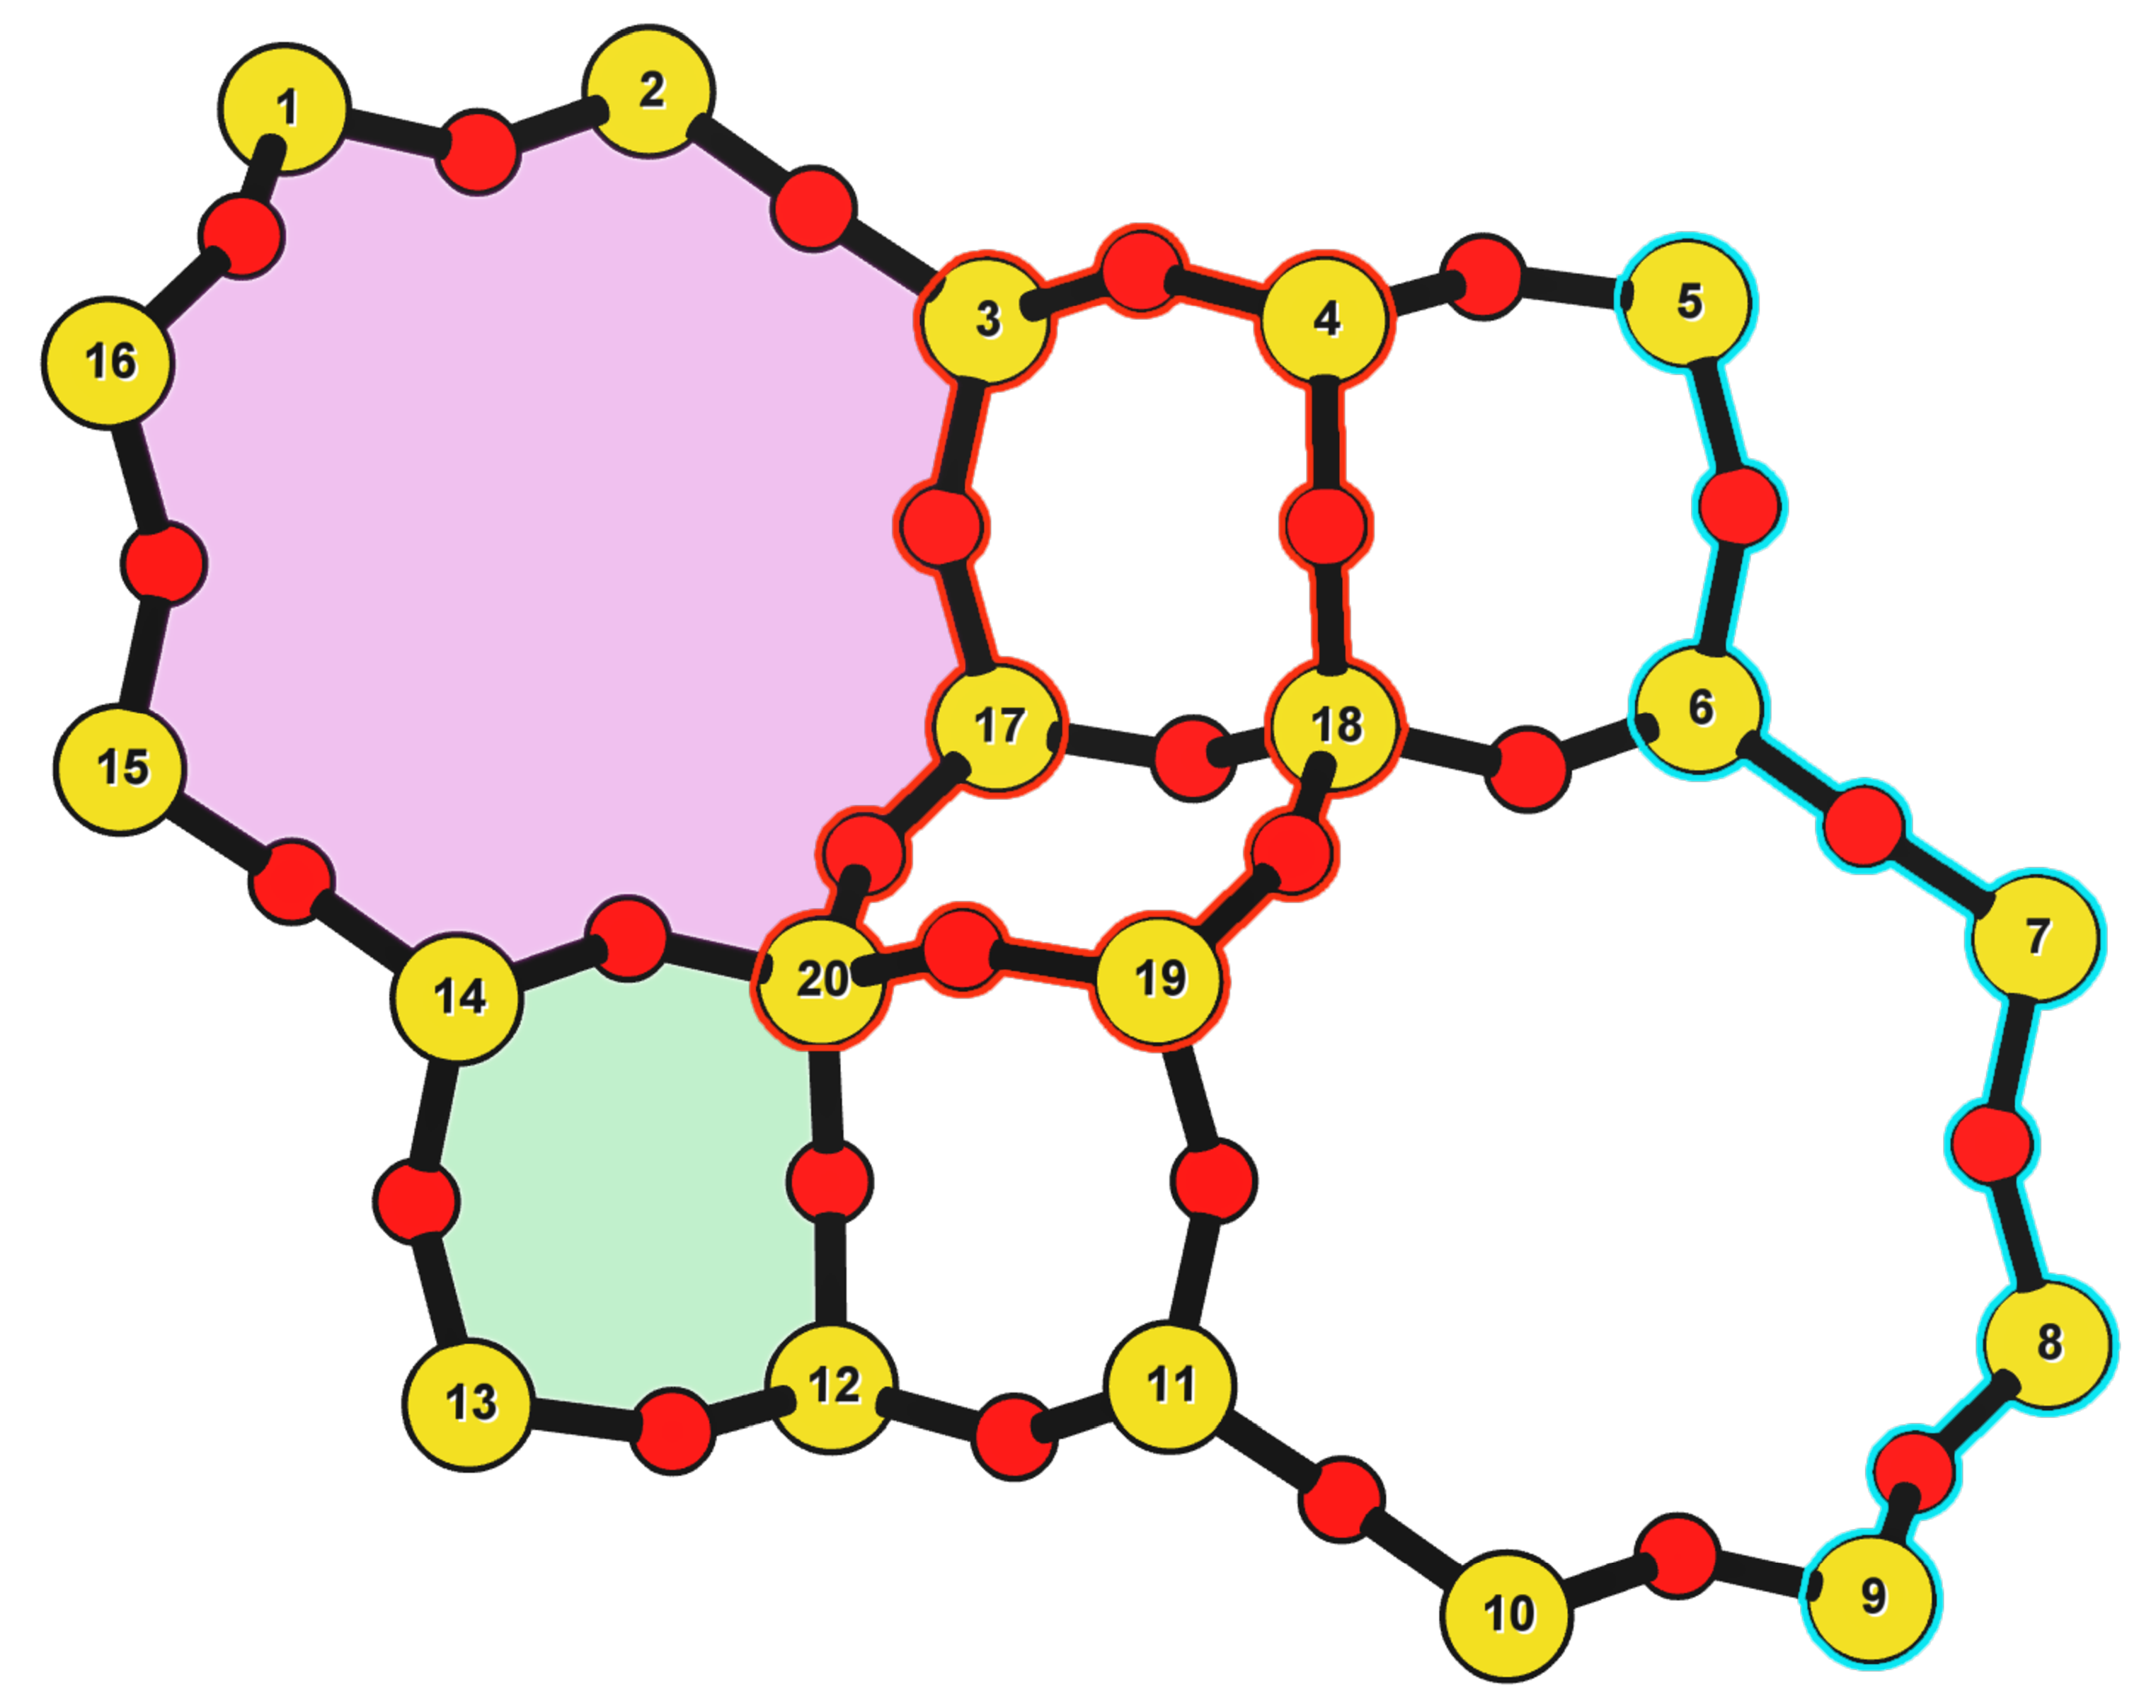
\includegraphics[width=0.60\textwidth]{../figures/completed-figures/ring-examples.pdf}
\captionof{figure}{Cutout of the Chabazite framework showing a path from node 3 to node 9 outlined in teal, a cycle (3-4-18-19-20-17) outlined in red, an 8-MR in pink, and a 4-MR in green. Yellow atoms are Si (T-sites), and red atoms are oxygen. \label{fig:cha-labeled}}
\end{center}

\newpage

\begin{longtable}{l p{2.7cm} p{2.7cm} p{2.7cm} p{2.7cm}}
\caption{Matrix showing relationship between frameoworks, nodes, paths, cycles, and various ring types. \red{Vertex symbol doesn't belong in the first column. It isn't a topological feature.} \label{tab:ring-def}}
\\
 & Description & Framework & Node (T-Sites) & Node (Oxygen)\\
\hline
\endfirsthead
\multicolumn{5}{l}{Continued from previous page} \\
\hline

 & Description & Framework & Node (T-Sites) & Node (Oxygen) \\

\hline
\endhead
\hline\multicolumn{5}{r}{Continued on next page} \\
\endfoot
\endlastfoot
\hline
Nodes & T-sites and oxygen atoms & Contains some set of symmetry distinct T-sites and oxygen atoms &  & \\
Paths & Collection of connected nodes from source to target & Periodic cell contains an infinite number of paths &  & \\
Cycles & Path that starts and ends at the same node & Periodic cell contains an infinite number of cycles &  & \\
Rings & Cycle that contains no shortcuts & Contains a finite number of unique rings & All rings that pass through particular T-site & All rings that pass through particular oxygen atom\\
Unstacked Rings & Ring that does not traverse two stacked rings & A subset of the Rings above & All unstacked rings that pass through T-site & All unstacked rings that pass through oxygen atom\\
Shortest Path Rings & Ring that is the shortest ring for at least one set of O-T-O on the cycle & A smaller subset of the rings above & All shortest path rings starting from a T-site (Vertex) & All shortest path rings that pass through oxygen atom\\
\red{Vertex Symbol} & Way to classify the rings around a T-site, shortest ring (and its multiplicity) for each O-O pair around a T-site & Collection of vertex symbols for all symmetry distinct T-sites in framework & Vertex symbol for particular T-site & \\
Geometric rings & A cycle that may contain a shortcut, but has similar geometric/chemical properties to a ring without a shortcut & Contains a finite number of geometric rings & Can be described by the geometric rings that pass through & Can be described by the geometric rings that pass through\\
\end{longtable}


\textbf{\textbf{Problem to address}}
\begin{itemize}
\item Different conventions exist that can reduce the set of rings to more strictly defined properties
\item These methods return different sets of rings
\item We can use rings to characterize oxygen atoms, T-sites, and entire frameworks
\item T-sites:
\begin{itemize}
\item Vertex symbols are the set of shortest paths connecting the 6 oxygen-oxygen pairs around a T-site \cite{okeeffe-vertex-1997}
\item Shortest path rings count all the vertex symbol rings that pass through a T-site or an oxygen atom \cite{sastre-topological-2009}
\item Or we can count all the rings that do not have a short cut \cite{goetzke-properties-1991}
\end{itemize}
\item Oxygen atoms:
\begin{itemize}
\item Shortest path rings
\item All rings with out a shortcut
\end{itemize}
\item Framework
\begin{itemize}
\item Vertex symbol rings
\item Shortest path rings
\item All rings with out a shortcut
\end{itemize}
\item Differences in ring counts leads to differences in how we describe the topology of zeolites. Therefore, when discussing the rings in a zeolite it is important to also state which method of ring counting is used.
\end{itemize}

\textbf{\textbf{Solution to problem}}
\begin{itemize}
\item Here we present Zeolite Simulation Environment (ZSE), a Python package that implements the ring finding algorithm presented by Goetzke and Klein \cite{goetzke-properties-1991} to find rings up to a user defined cutoff size, and can implement the previously published ring set reduction conventions.
\item We use ZSE to provide an analysis of rings using each of these conventions on the entire set of IZA zeolite frameworks to compare how they result in different characterizations
\end{itemize}

\red{Introduction needs to foreshadow the important insights. We captured those in your abstract. They need to appear here too.}

Using ZSE we show the differences in framework, T-site, and oxygen ring descriptors when using the various ring counting conventions. We highlight rings that are found by these conventions but not typically discussed for a number of frameworks. We also show that the vertex symbol, a common approach used to characterize T-sites misses important parts of the stereochemistry around a T-site. 


\section*{Software Description}
\label{sec:orgb3ae4e5}

\begin{itemize}
\item All of the frameworks listed on the IZA Database of zeolite structures \cite{baerlocher-database-nodate} are included in a database with ZSE
\item These structures are Atomic Simulation Environment Atoms objects \cite{larsen-atomic-2017}, and can be used with any of the functions in ZSE
\item ZSE also includes CIF tools to read structure files for frameworks not listed in the IZA website, such as hypothetical zeolites, and return an Atoms object that can be used with ZSE
\item ZSE has 3 previously published rules for ring finding implemented
\begin{itemize}
\item All cycles without a shortcut \cite{goetzke-properties-1991}
\item All shortest path cycles \cite{sastre-topological-2009}
\item Cycles that compose the vertex symbol for a T-site \cite{okeeffe-vertex-1997}
\end{itemize}
\item We have also implemented a new rule that finds all rings with out a shortcut, but excludes rings that are made by traversing a stacked set of rings. \red{Have to define stacked ring.}
\begin{itemize}
\item Figure showing example of 8-MR in the d6r of CHA and 14-MR in AFI
\end{itemize}
\item Each of the rules: shortest path, vertex symbols, and our new rule are a subset of the no shortcuts rule
\end{itemize}
Process to find rings:
\begin{enumerate}
\item To find rings in a zeolite, ZSE makes a custom connectivity matrix for the Si and O atoms in the framework
\item We use NetworkX \cite{hagberg-exploring-2008} to build a shortest path matrix for every atom pair in the zeolite framework
\item We then find all the rings up to some cutoff size base on the algorithm presented by Goetzke and Klein \cite{goetzke-properties-1991}
\item Depending on the rule chosen by the user, ZSE then removes rings from this list that don't meet the qualifications of the rule
\item ZSE returns a list of the rings found, a list of the atom indicies that compose each ring, Atoms objects for each ring that can be further analyzed or visualized by the user
\end{enumerate}


\section*{Results}
\label{sec:orgc51c807}
\begin{itemize}
\item Ring counts frequency plots
\begin{itemize}
\item Plot showing how many frameworks on the IZA contain each size ring found using the various ring counting methods
\item This highlights the differences in the ring rules, and shows that results will vary depending on rule.
\end{itemize}
\end{itemize}
\begin{center}
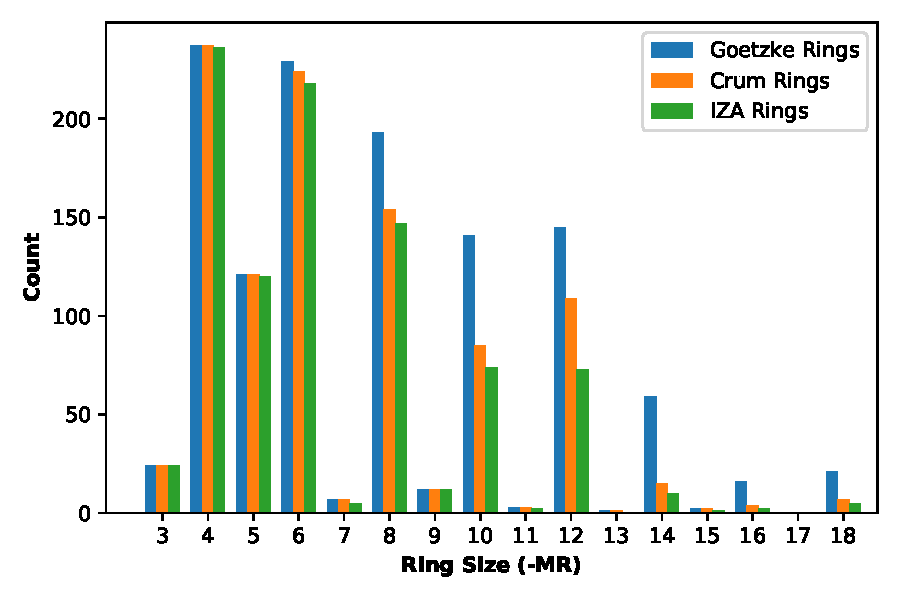
\includegraphics[width=.6\textwidth]{../figures/completed-figures/ring-counts.pdf}
\captionof{figure}{Number of IZA frameworks containing each size ring, using the various ring counting rules. [This will be updated with the Sastre method, vertex method, and the rings listed on  the IZA website. Currently the IZA does not show any ring data for the SVY framework, providing one less framework to count.  \label{fig:ring-counts}}
\end{center}

\begin{itemize}
\item Number of unique T-sites
\begin{itemize}
\item There are 1460 T-sites through all the frameworks listed on the IZA website.
\item We can characterize those T-sites by the rings that pass through them
\item Sastre did this, and called the list of rings, the ring index
\item If we do this using different rules for ring finding how do the results change?
\begin{itemize}
\item See \Cref{fig:unique-ts}
\end{itemize}
\item Most common T-site ring index using Goetzke method is: 5\(_{\text{6}}\)\textbullet{}10\(_{\text{4}}\) showing up 23 times through the IZA frameworks.
\item Most common T-site ring index using Crum method is: 4\(_{\text{3}}\)\textbullet{}8\(_{\text{4}}\) showing up 31 times through the IZA frameworks.
\begin{itemize}
\item Next most common T-site with Crum method is 5\(_{\text{6}}\)\textbullet{}10\(_{\text{4}}\) showing up 25 times
\end{itemize}
\item This raises the question, if you want to use machine learning to correlate T-site rings to chemical properties, which ring method should you use?
\end{itemize}
\end{itemize}
\begin{center}
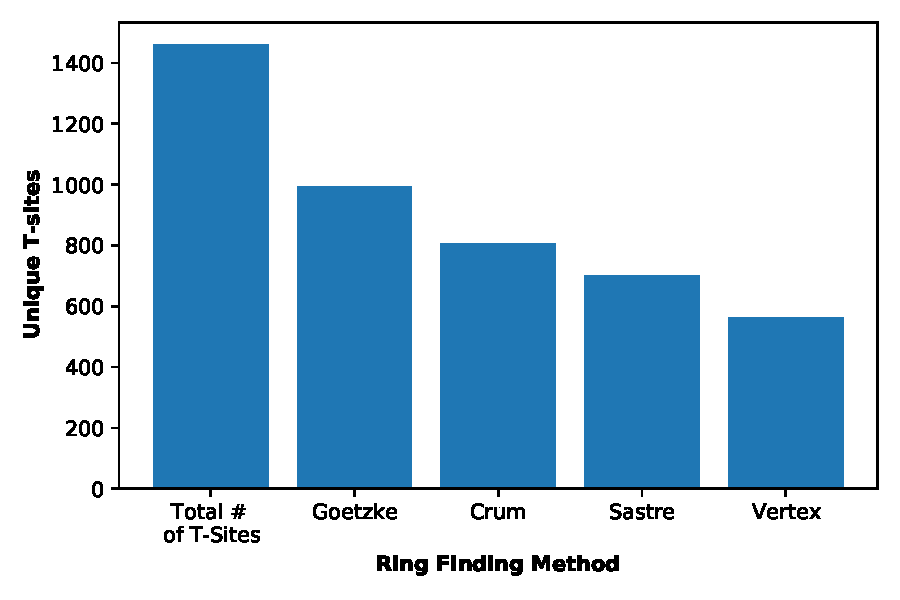
\includegraphics[width=.6\textwidth]{../figures/completed-figures/unique-ts.pdf}
\captionof{figure}{Number of unique T-sites when classified by the rings passing through them using varrious ring finding rules. \label{fig:unique-ts}}
\end{center}

\begin{itemize}
\item Number of unique oxygen sites
\begin{itemize}
\item We can repeat this method for the oxygen atoms in all the frameworks
\item Counting the symmetry distinct oxygen atoms in each framework on the IZA database leads to a total count of 3219
\item We can classify those oxygen atoms based on the rings that pass through them, using the various ring counting rules
\item \Cref{fig:unique-os} shows counts based on ring finding rules
\item The percentage of unique oxygen sites is much lower than the percentage of unique T-sites for every ring finding method
\end{itemize}
\end{itemize}

\begin{center}
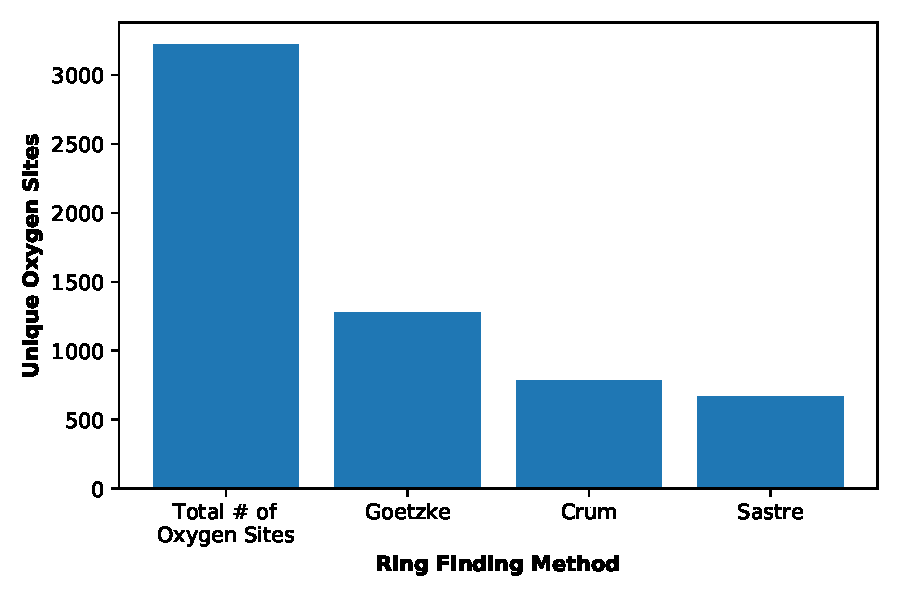
\includegraphics[width=.6\textwidth]{../figures/completed-figures/unique-os.pdf}
\captionof{figure}{Number of unique oxygen sites when classified by the rings passing through them using varrious ring finding rules. Vertex method not included, since that is a way to classify T-sites only. \label{fig:unique-os}}
\end{center}

\begin{itemize}
\item Reproduce the results from Sastre paper, show ring counts with the other rules, \Cref{tab:ring-counts}
\begin{itemize}
\item Ring index was presented by Sastre and Corma as a way to list the rings that pass through a node in a zeolite \cite{sastre-topological-2009}
\item List rings from smallest to largest, and any multiplicities are shown by a subscript
\item This is a convenient way to characterize the atoms of a zeolite by the rings they are associated with
\item Results in the Sastre column were found using ZSE but agree directly with the results shown by Sastre and Corma \cite{sastre-topological-2009}
\item This provides an in depth look at some of the frameworks and the differences in rings found by each rule.
\item Leads into the next section discussing the specific rings of CHA and pentasil that do or don't get counted by each rule.
\end{itemize}
\end{itemize}

\begin{table}[htbp]
\caption{Comparison of Ring Indices for the T-sites in Various Uninodal Zeolite Frameworks \label{tab:ring-counts}}
\centering
\begin{tabular}{llll}
Framework & Goetzke & Crum & Sastre \cite{sastre-topological-2009}\\
\hline
ABW & 4\(_{\text{2}}\)\textbullet{}6\(_{\text{3}}\)\textbullet{}8\(_{\text{4}}\) & 4\(_{\text{2}}\)\textbullet{}6\(_{\text{3}}\)\textbullet{}8\(_{\text{4}}\) & 4\(_{\text{2}}\)\textbullet{}6\(_{\text{3}}\)\textbullet{}8\(_{\text{4}}\)\\
ACO & 4\(_{\text{3}}\)\textbullet{}6\(_{\text{3}}\)\textbullet{}8\(_{\text{6}}\)\textbullet{}10\(_{\text{15}}\) & 4\(_{\text{3}}\)\textbullet{}8\(_{\text{6}}\) & 4\(_{\text{3}}\)\textbullet{}8\(_{\text{6}}\)\\
AFI & 4\(_{\text{1}}\)\textbullet{}6\(_{\text{13}}\)\textbullet{}12\(_{\text{1}}\)\textbullet{}14\(_{\text{7}}\) & 4\(_{\text{1}}\)\textbullet{}6\(_{\text{13}}\)\textbullet{}12\(_{\text{1}}\) & 4\(_{\text{1}}\)\textbullet{}6\(_{\text{13}}\)\\
ANA & 4\(_{\text{2}}\)\textbullet{}6\(_{\text{2}}\)\textbullet{}8\(_{\text{16}}\) & 4\(_{\text{2}}\)\textbullet{}6\(_{\text{2}}\)\textbullet{}8\(_{\text{16}}\) & 4\(_{\text{2}}\)\textbullet{}6\(_{\text{2}}\)\textbullet{}8\(_{\text{16}}\)\\
ATO & 4\(_{\text{1}}\)\textbullet{}6\(_{\text{9}}\)\textbullet{}8\(_{\text{8}}\)\textbullet{}12\(_{\text{20}}\) & 4\(_{\text{1}}\)\textbullet{}6\(_{\text{9}}\)\textbullet{}12\(_{\text{20}}\) & 4\(_{\text{1}}\)\textbullet{}6\(_{\text{9}}\)\\
BCT & 4\(_{\text{1}}\)\textbullet{}6\(_{\text{6}}\)\textbullet{}8\(_{\text{20}}\) & 4\(_{\text{1}}\)\textbullet{}6\(_{\text{6}}\)\textbullet{}8\(_{\text{12}}\) & 4\(_{\text{1}}\)\textbullet{}6\(_{\text{6}}\)\\
CHA & 4\(_{\text{3}}\)\textbullet{}6\(_{\text{1}}\)\textbullet{}8\(_{\text{6}}\)\textbullet{}12\(_{\text{1}}\) & 4\(_{\text{3}}\)\textbullet{}6\(_{\text{1}}\)\textbullet{}8\(_{\text{2}}\)\textbullet{}12\(_{\text{1}}\) & 4\(_{\text{3}}\)\textbullet{}6\(_{\text{1}}\)\textbullet{}8\(_{\text{2}}\)\\
DFT & 4\(_{\text{2}}\)\textbullet{}6\(_{\text{6}}\)\textbullet{}8\(_{\text{10}}\)\textbullet{}10\(_{\text{10}}\) & 4\(_{\text{2}}\)\textbullet{}6\(_{\text{6}}\)\textbullet{}8\(_{\text{10}}\) & 4\(_{\text{2}}\)\textbullet{}6\(_{\text{6}}\)\textbullet{}8\(_{\text{10}}\)\\
GIS & 4\(_{\text{3}}\)\textbullet{}8\(_{\text{4}}\) & 4\(_{\text{3}}\)\textbullet{}8\(_{\text{4}}\) & 4\(_{\text{3}}\)\textbullet{}8\(_{\text{4}}\)\\
GME & 4\(_{\text{3}}\)\textbullet{}6\(_{\text{1}}\)\textbullet{}8\(_{\text{6}}\)\textbullet{}12\(_{\text{7}}\) & 4\(_{\text{3}}\)\textbullet{}6\(_{\text{1}}\)\textbullet{}8\(_{\text{2}}\)\textbullet{}12\(_{\text{1}}\) & 4\(_{\text{3}}\)\textbullet{}6\(_{\text{1}}\)\textbullet{}8\(_{\text{2}}\)\\
MER & 4\(_{\text{3}}\)\textbullet{}8\(_{\text{4}}\)\textbullet{}10\(_{\text{10}}\)\textbullet{}14\(_{\text{14}}\) & 4\(_{\text{3}}\)\textbullet{}8\(_{\text{4}}\) & 4\(_{\text{3}}\)\textbullet{}8\(_{\text{4}}\)\\
MON & 4\(_{\text{1}}\)\textbullet{}5\(_{\text{5}}\)\textbullet{}8\(_{\text{6}}\) & 4\(_{\text{1}}\)\textbullet{}5\(_{\text{5}}\)\textbullet{}8\(_{\text{6}}\) & 4\(_{\text{1}}\)\textbullet{}5\(_{\text{5}}\)\textbullet{}8\(_{\text{6}}\)\\
NPO & 3\(_{\text{1}}\)\textbullet{}6\(_{\text{6}}\)\textbullet{}12\(_{\text{40}}\) & 3\(_{\text{1}}\)\textbullet{}6\(_{\text{6}}\)\textbullet{}12\(_{\text{40}}\) & 3\(_{\text{1}}\)\textbullet{}6\(_{\text{6}}\)\\
\end{tabular}
\end{table}


\begin{itemize}
\item Here we show the most common ring indices for T-sites in the IZA database using each of the ring finding rules
\item \Cref{tab:goetzke-ts} shows the five most common ring indices for T-sites using the Goetzke  rule
\end{itemize}
\begin{table}[htbp]
\caption{Most Common Ring Indices Using the Goetzke Rule \label{tab:goetzke-ts}}
\centering
\begin{tabular}{lrl}
Ring Index & Count & Frameworks Containing Index\\
\hline
5\(_{\text{6}}\)\textbullet{}10\(_{\text{4}}\) & 23 & IMF(2), MEL(1), MFI(2), PRO(1),\\
 &  & SVR(2), TUN(2), SFV(13)\\
4\(_{\text{1}}\)\textbullet{}5\(_{\text{3}}\)\textbullet{}6\(_{\text{2}}\)\textbullet{}10\(_{\text{3}}\)\textbullet{}12\(_{\text{4}}\) & 14 & MEL(1), SFV(13)\\
4\(_{\text{1}}\)\textbullet{}5\(_{\text{3}}\)\textbullet{}6\(_{\text{2}}\)\textbullet{}8\(_{\text{5}}\)\textbullet{}10\(_{\text{1}}\) & 14 & MEL(1), SFV(13)\\
5\(_{\text{5}}\)\textbullet{}6\(_{\text{3}}\)\textbullet{}10\(_{\text{1}}\)\textbullet{}12\(_{\text{1}}\) & 14 & MEL(1), SFV(13)\\
5\(_{\text{4}}\)\textbullet{}6\(_{\text{3}}\)\textbullet{}8\(_{\text{2}}\)\textbullet{}10\(_{\text{3}}\) & 14 & MEL(1), SFV(13)\\
\end{tabular}
\end{table}

\newpage
\begin{itemize}
\item \Cref{tab:crum-ts} shows the five most common ring indices for T-sites using the Crum rule
\end{itemize}
\begin{table}[htbp]
\caption{Five Most Common Ring Indices Using the Crum Rule \label{tab:crum-ts}}
\centering
\begin{tabular}{lrl}
Ring Index & Count & Frameworks Containing Index\\
\hline
4\(_{\text{3}}\)\textbullet{}8\(_{\text{4}}\) & 31 & APC(1), GIS(1), MER(1), MWF(13),\\
 &  & PAU(6), PHI(2), PWN(2), SIV(4)\\
5\(_{\text{6}}\)\textbullet{}10\(_{\text{4}}\) & 25 & IMF(3), MEL(1), MFI(2), RRO(1),\\
 &  & SVR(2), TUN(3), SFV(13)\\
4\(_{\text{2}}\)\textbullet{}6\(_{\text{4}}\) & 17 & FAR(1), FRA(6), GIU(1), LIO(1),\\
 &  & LOS(2), LTN(2), MAR(1), SOD(1),\\
 &  & TOL(2)\\
5\(_{\text{5}}\)\textbullet{}6\(_{\text{3}}\)\textbullet{}10\(_{\text{1}}\) & 17 & IMF(1), MEL(1), MFI(1), TUN(1),\\
 &  & SFV(13)\\
4\(_{\text{3}}\)\textbullet{}6\(_{\text{1}}\)\textbullet{}8\(_{\text{2}}\)\textbullet{}12\(_{\text{1}}\) & 16 & AFS(1), AFT(3), AFV(1), AFX(2),\\
 &  & AVL(2), BPH(1), CHA(1), GME(1),\\
 &  & SBE(1), SFW(3)\\
\end{tabular}
\end{table}

\begin{itemize}
\item \Cref{tab:sastre-ts} shows the five most common ring indices for T-sites using the Sastre rule
\end{itemize}
\begin{table}[htbp]
\caption{Five Most Common Ring Indices Using the Sastre Rule \label{tab:sastre-ts}}
\centering
\begin{tabular}{lrl}
Ring Index & Count & Frameworks Containing Index\\
\hline
4\(_{\text{2}}\)\textbullet{}6\(_{\text{4}}\) & 39 & AFG(3), CAN(1), FAR(4), FRA(6),\\
 &  & GIU(5), LIO(4), LOS(2), LTN(2)\\
 &  & MAR(4), SOD(1), TOL(7)\\
5\(_{\text{6}}\)\textbullet{}10\(_{\text{4}}\) & 33 & IMF(3), MEL(2), MFI(2), RRO(1),\\
 &  & SVR(2), TUN(2), SFV(21)\\
4\(_{\text{3}}\)\textbullet{}8\(_{\text{4}}\) & 30 & GIS(1), MER(1), MWF(14), PAU(6),\\
 &  & PHI(2), PWN(2), SIV(4)\\
4\(_{\text{3}}\)\textbullet{}6\(_{\text{1}}\)\textbullet{}8\(_{\text{2}}\) & 28 & AEI(3), AFT(3), AFV(1), AFX(2),\\
 &  & AVL(2), CHA(1), GME(1), KFI(1),\\
 &  & LTF(1), MWF(2), PAU(2), PWN(1),\\
 &  & RHO(1), SAV(3), SFW(3), TSC(1)\\
4\(_{\text{3}}\)\textbullet{}6\(_{\text{2}}\)\textbullet{}8\(_{\text{1}}\) & 24 & AFV(1), AVE(2), AVL(1), CLO(2),\\
 &  & EAB(1), ERI(1), IFY(1), IRN(1),\\
 &  & LEV(1), LTA(1), LTN(1), MOZ(1),\\
 &  & OFF(1), SAT(1), SWY(2), TSC(1),\\
 &  & UFI(1), PTT(1), SYT(3)\\
\end{tabular}
\end{table}

\begin{itemize}
\item \Cref{tab:vertex-ts} shows the five most common ring indices for T-sites using vertex symbols
\end{itemize}
\begin{table}[htbp]
\caption{Five Most Common Ring Indices Using Vertex Symbolscite:bernauer-proton-2016 \label{tab:vertex-ts}}
\centering
\begin{tabular}{lrl}
Vertex Symbol & Count & Frameworks Containing Index\\
\hline
4\textbullet{}4\textbullet{}6\textbullet{}6\textbullet{}6\textbullet{}6 & 40 & AFG(3), CAN(1), FAR(4), FRA(6),\\
 &  & GIU(5), LIO(4), LOS(2), LTN(2),\\
 &  & MAR(4), RON(1), SOD(1), TOL(7)\\
4\textbullet{}4\textbullet{}4\textbullet{}6\textbullet{}8\textbullet{}8 & 32 & AEI(3), AFT(3), AFV(1), AFX(2),\\
 &  & ATT(1), AVL(2), CHA(1), ETV(1),\\
 &  & GME(1), KFI(1), LTF(1), MRT(2),\\
 &  & MWF(2), PAU(2), PWN(1), RHO(1),\\
 &  & SAV(3), SFW(3), TSC(1)\\
4\textbullet{}4\textbullet{}4\textbullet{}6\textbullet{}6\textbullet{}8 & 30 & AFV(1), AVE(2), AVL(1), CGS(1),\\
 &  & CLO(2), EAB(1), ERI(1), ETR(1),\\
 &  & IFY(1), IRN(1), JSW(1), LEV(1),\\
 &  & LTA(1), LTL(1), LTN(1), MOZ(3),\\
 &  & OFF(1), PTT(1), SAT(1), SWY(2),\\
 &  & SYT(3), TSC(1), UFI(1)\\
4\textbullet{}4\textbullet{}4\textbullet{}8\textbullet{}8\textbullet{}8\(_{\text{2}}\) & 30 & GIS(1), MER(1), MWF(14), PAU(6),\\
 &  & PHI(2), PWN(2), SIV(4)\\
5\textbullet{}5\textbullet{}5\textbullet{}5\textbullet{}5\textbullet{}6 & 26 & DDR(1), DOH(2), IHW(1), IMF(1),\\
 &  & MEL(1), MEP(1), MFI(1), MTN(1),\\
 &  & SFS(1), SFV(15), TUN(1)\\
\end{tabular}
\end{table}

\newpage

\begin{itemize}
\item These ring finding rules often find rings that are not commonly discussed in literature, and are not listed by the IZA
\item These are classified as untabulated rings by Curtis and Deem \cite{curtis-statistical-2003}
\item However it is possible that these rings are relevant for describing chemical, catalytic, or topological properties of zeolites
\item Here we show an example of untabulated rings in the Chabazite framework
\item Show the cage belts results for CHA, AFT, etc\ldots{} and discuss how those rings don't show up in previous literature, \Cref{fig:cha-rings}
\begin{itemize}
\item Looking at results for CHA in \Cref{tab:ring-counts} we see the Goetzke method finds 4\(_{\text{3}}\)\textbullet{}6\(_{\text{1}}\)\textbullet{}8\(_{\text{6}}\)\textbullet{}12\(_{\text{1}}\)
\item This is different from the results in the Sastre paper \cite{sastre-topological-2009}, in that they only show 2 8-MRs and no 12-MRs
\item The extra 8-MRs result from cycles traversing nodes in both 6-MRs of the d6r
\begin{itemize}
\item Crum rule removes these 8-MRs while still finding the 12-MR
\item Sastre rule does not find the 8-MRs in the d6r or the 12-MR
\end{itemize}
\item The 12-MR is a cycle that circumferences the CHA cage
\end{itemize}
\end{itemize}
\begin{center}
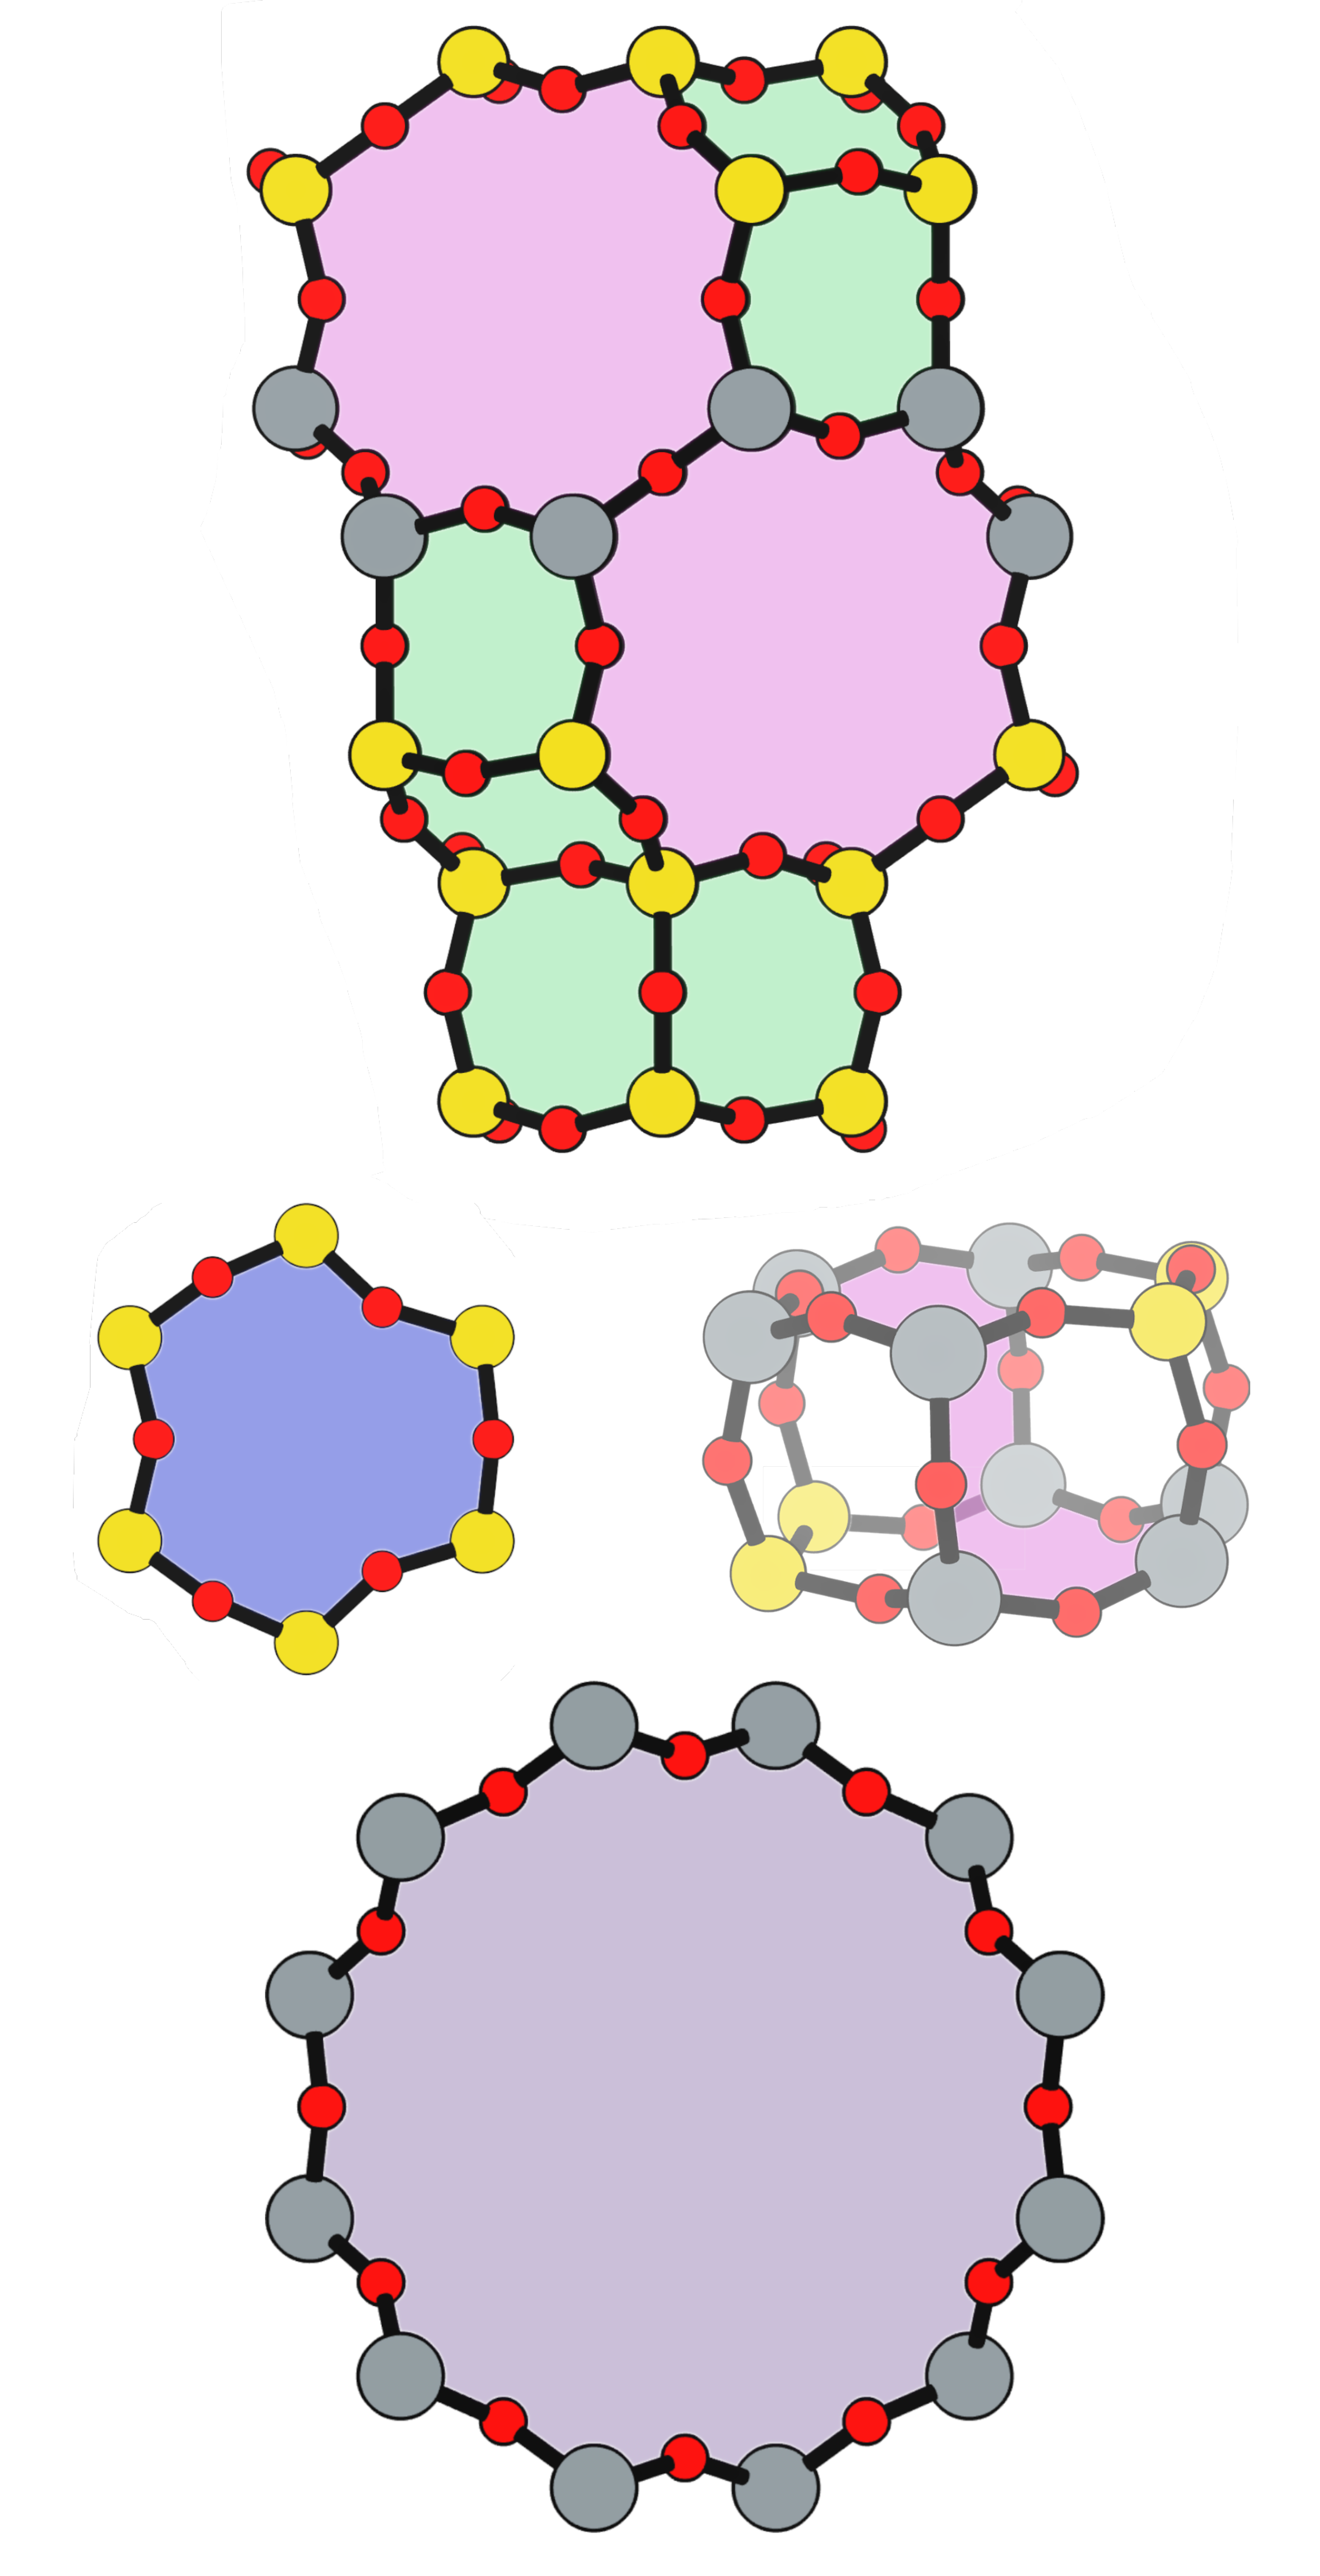
\includegraphics[width=0.45\textwidth]{../figures/completed-figures/cha-all-rings.pdf}
\captionof{figure}{Chabazite cage and d6r with highlighted rings: 4-MR in green, 8-MR in pink, and 12-MR in purple. The 8-MR in the d6r and the 12-MR are rings not typically discussed in literature, Si atoms have been replaced with Al atoms to help identify those rings in the overall cage structure.. \label{fig:cha-rings}}
\end{center}

\begin{itemize}
\item On the other end of the spectrum, there are cycles that would not be classified as a rings by the connectivity rules previously outlined that display properties similar to rings
\item These shortcut containing cycles can display chemical and/or geometric properties consistent with rings, and are of interest to catalysis researchers even though they are not considered rings by connectivity rules
\item One example is the 6-membered cycle referred to as the \(\alpha\)-6-MR in literature (\Cref{fig:mfi-6}) and is present in a number of frameworks including but not limited to  MOR, FER, MFI, and BEA \cite{dedecek-siting-2012,bernauer-proton-2016}, which is a potential location for Co\(^{\text{2+}}\) uptake when two Al atoms are 3rd nearest neighbor in the cycle. Similar to Co\(^{\text{2+}}\) uptake in 3NN Al atoms in 6-MRs in other frameworks such as CHA and AEI.
\item This 6-membered cycle would not be considered a ring by any of the connectivity rules outlined here due to the shortcut splitting the cycle into two 5-MRs
\end{itemize}

\begin{center}
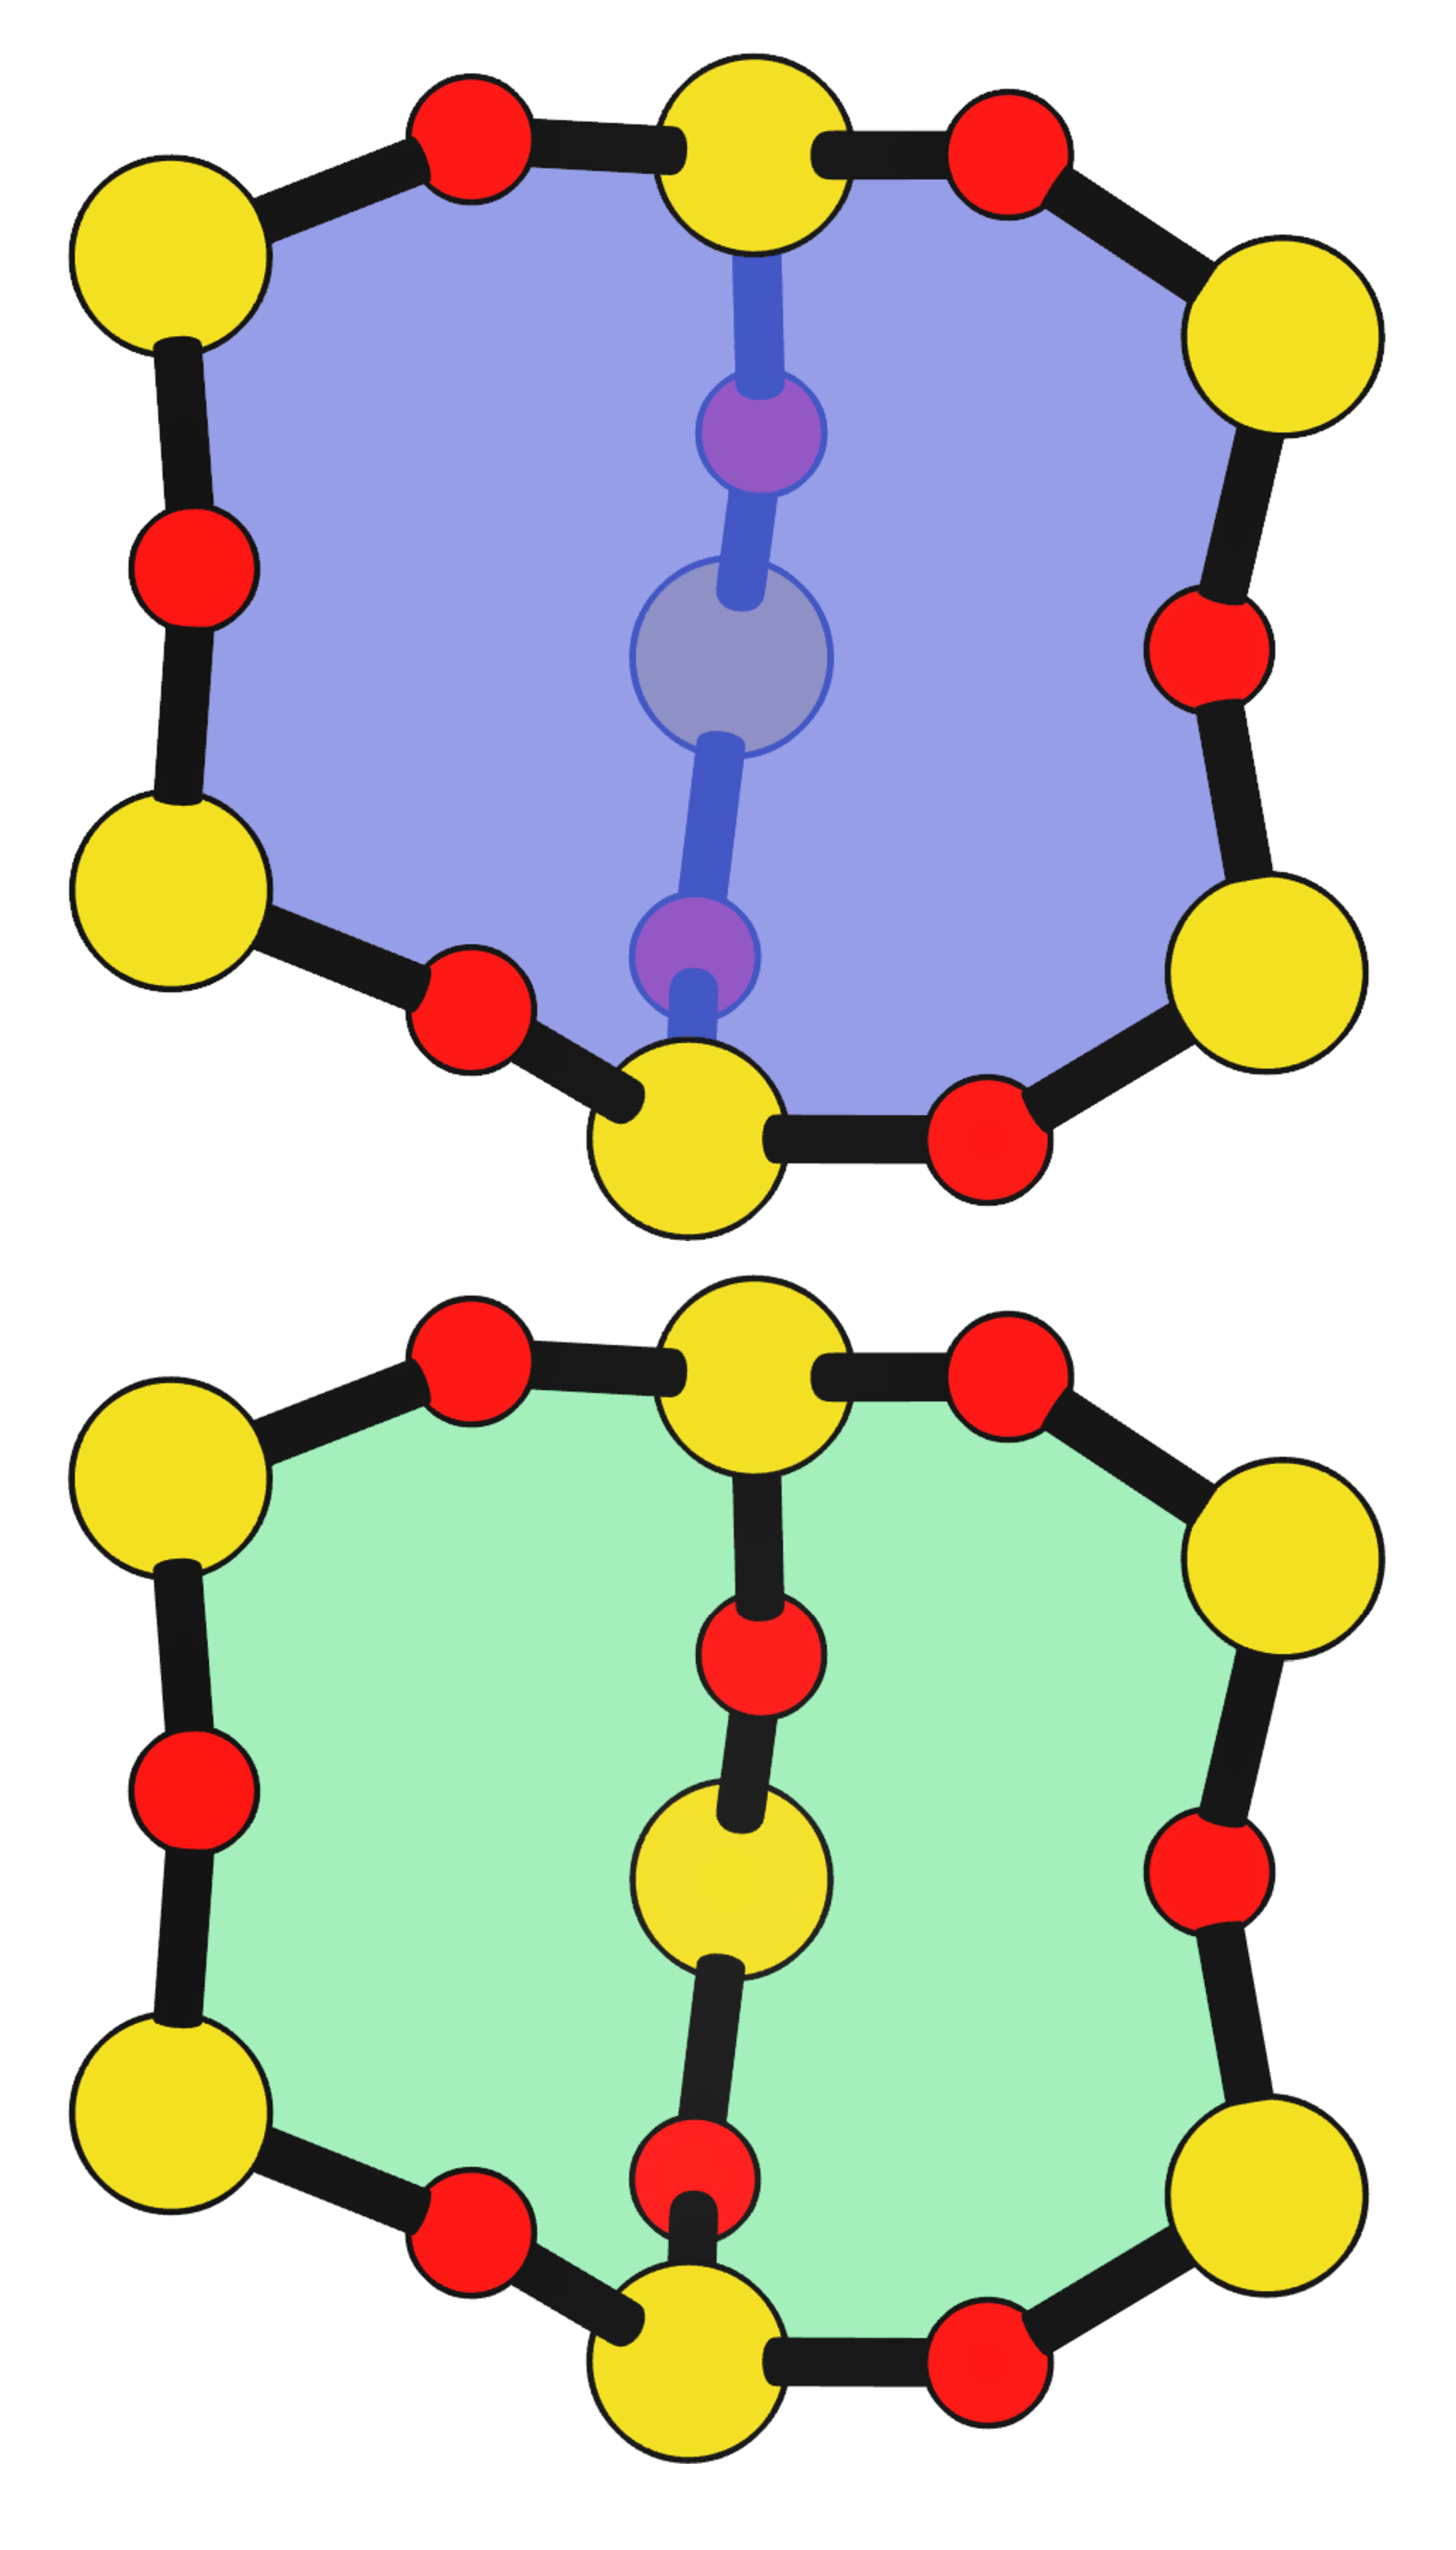
\includegraphics[width=.4\textwidth]{../figures/completed-figures/MFI-6MC.pdf}
\captionof{figure}{Cutout of MFI framework showing the structure referred to as an \(\alpha\)-6-MR in blue, and the two 5-MRs that compose it in green. The 6-membered cycle would not be found as a ring by any of the connectivity ring rules (Goetzke, Crum, Sastre, or vertex symbol). \label{fig:mfi-6}}
\end{center}


\section*{Conclusions}
\label{sec:org8668819}
\begin{itemize}
\item \red{Rings of graph are well defined; here identify all rings up to XXX in YYY frameworks. Find that commonly reported (IZA) ring sizes miss certain rings.}
\end{itemize}


\begin{itemize}
\item The method used to find rings in a zeolite will provide different ring counts \red{unclear}
\item When discussing rings in a zeolite it is import to disclose by which method those rings were found
\item Using ZSE we can find rings based on various methods
\item This provides a foundation for using ring fingerprints in machine learning models to correlate chemical properties and topology
\end{itemize}


\bibliographystyle{unsrtnat}
\bibliography{ref}

\section*{Acknowledgments}
\label{sec:orgf0794ce}
\begin{itemize}
\item Funding
\begin{itemize}
\item CISTAR
\item Schmitt Fellowship
\end{itemize}
\item Discussions
\begin{itemize}
\item Christian Baerlocher
\end{itemize}
\item Software:
\begin{itemize}
\item German Sastre: zeoTsites
\end{itemize}
\item Compute Resources
\begin{itemize}
\item CRC
\end{itemize}
\end{itemize}
\end{document}